\section{Example using URDAD with UML as modeling language}

This is an example of using the URDAD design methodology with UML as modeling
language to analyze the requirements and design a technology neutral business
process for the use case of a loan provider processing a loan application in order
to provide a loan. The design is technology neutral and can be mapped onto manual
implementations realized by people or onto automated implementations realized
within systems.

%===========================

\subsection{Analysis}

The first step is to identify the stake holders who have an interest in the use
case and then, for each stake holder, the functional requirements for that use case
as shown in figure \ref{fig:provideLoanFunctionalRequirements}. Note that we include
only the first level granularity functional requirements, not the functional requirements
of functional requirements. We have thus fixed the level of granularity.

\begin{figure}
  \centering
  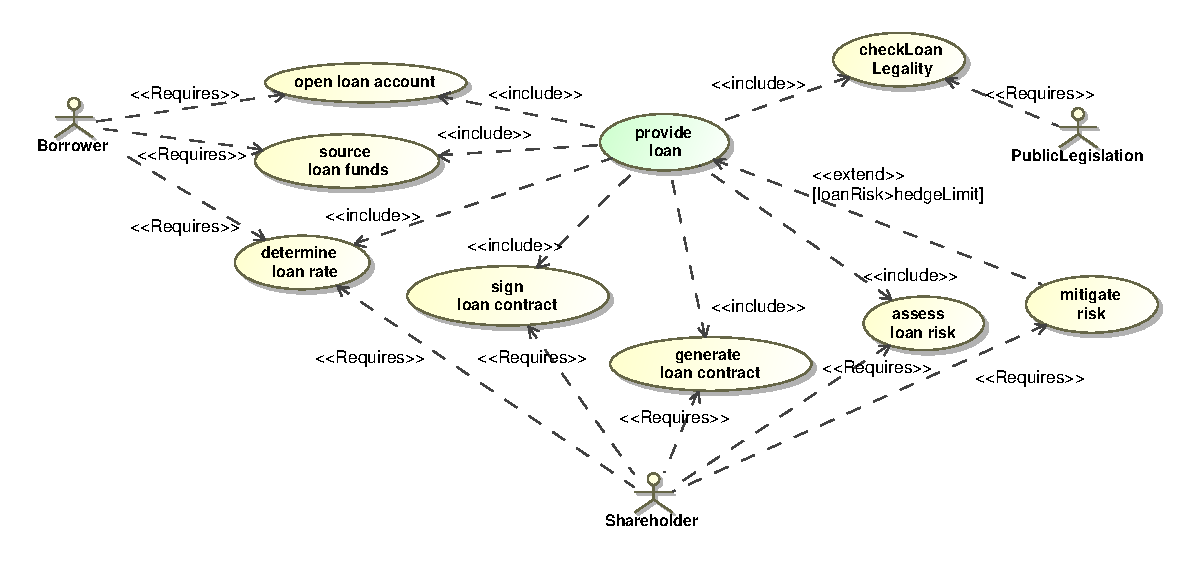
\epsfig{file=provideLoanFunctionalRequirements.eps, scale=0.6}
  \caption{Functional requirements for provide loan use case.}
  \label{fig:provideLoanFunctionalRequirements}
\end{figure}

Since this is the first level of granularity, we need to specify the user work
flow. This will contain the messages exchanged between the user and the
service provider for the various scenarios as shown in figure
\ref{fig:provideLoanUserWorkflow}.

\begin{figure}
  \centering
  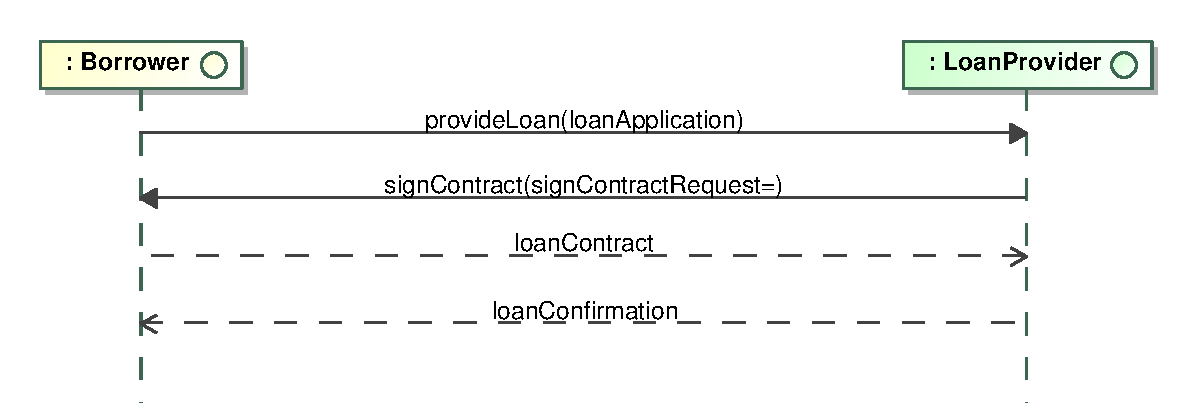
\epsfig{file=provideLoanUserWorkflow.eps, scale=0.6}
  \caption{User work flow.}
  \label{fig:provideLoanUserWorkflow}
\end{figure}

We need to add class diagrams specifying the information which must be
contained in the exchanged value objects. At this stage the class diagrams
will only specify the information as required, at this level of granularity,
 by the stake holders. As the
business process design is taken through levels of granularity, one will
typically add identify further structure which needs to be added to these classes.

In order to define a formal services contract for the use case we specify the
pre- and post-conditions and quality requirements. In practice the pre- and
post-conditions would be assembled in OCL across other services specified
for that service provider. The quality requirements can be formalized using the
{\em UML Profile for Modeling Quality of Service and Fault Tolerance Characteristics
and Mechanisms} \cite{omg:umlProfileQos}. The informal services contract is shown
in figure \ref{fig:provideLoanContract}.

\begin{figure}
  \centering
  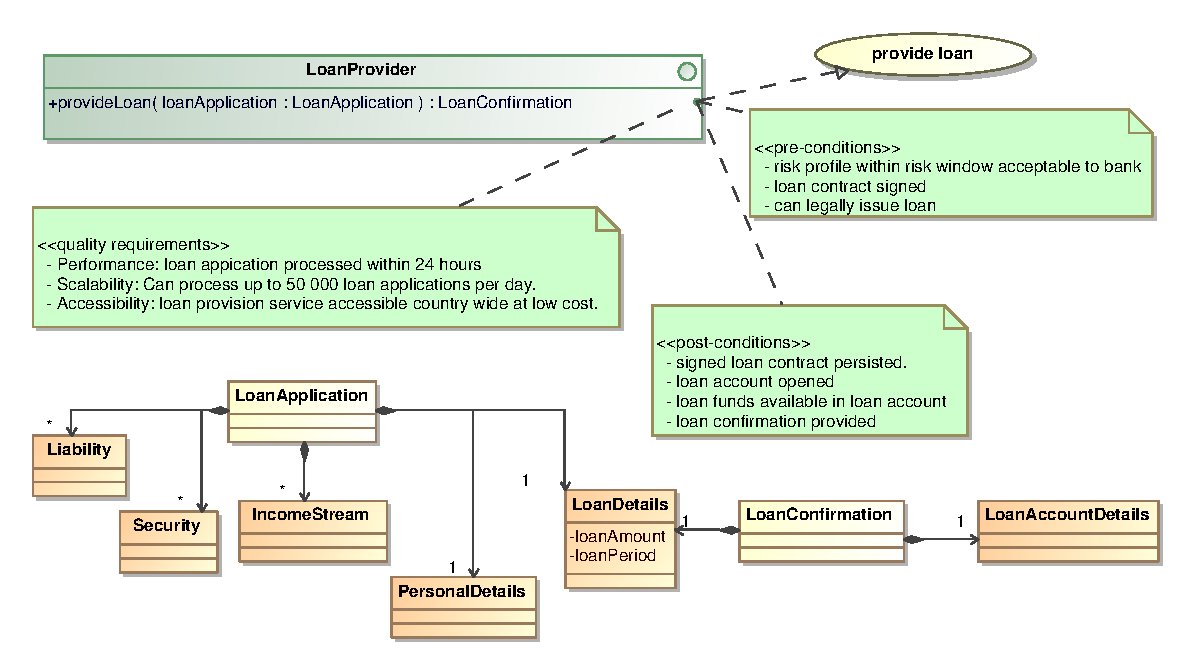
\epsfig{file=provideLoanContract.eps, scale=0.6}
  \caption{Services contract for the provide loan service.}
  \label{fig:provideLoanContract}
\end{figure}

%=============================================================

\subsection{Business process design}


The first step of the design phase is that of grouping functional requirements
into responsibility domains and assigning each responsibility domain to a
separate services contract. The result of this is shown in figure
\ref{fig:provideLoanResponsibilityAllocation}.

\begin{figure}
  \centering
  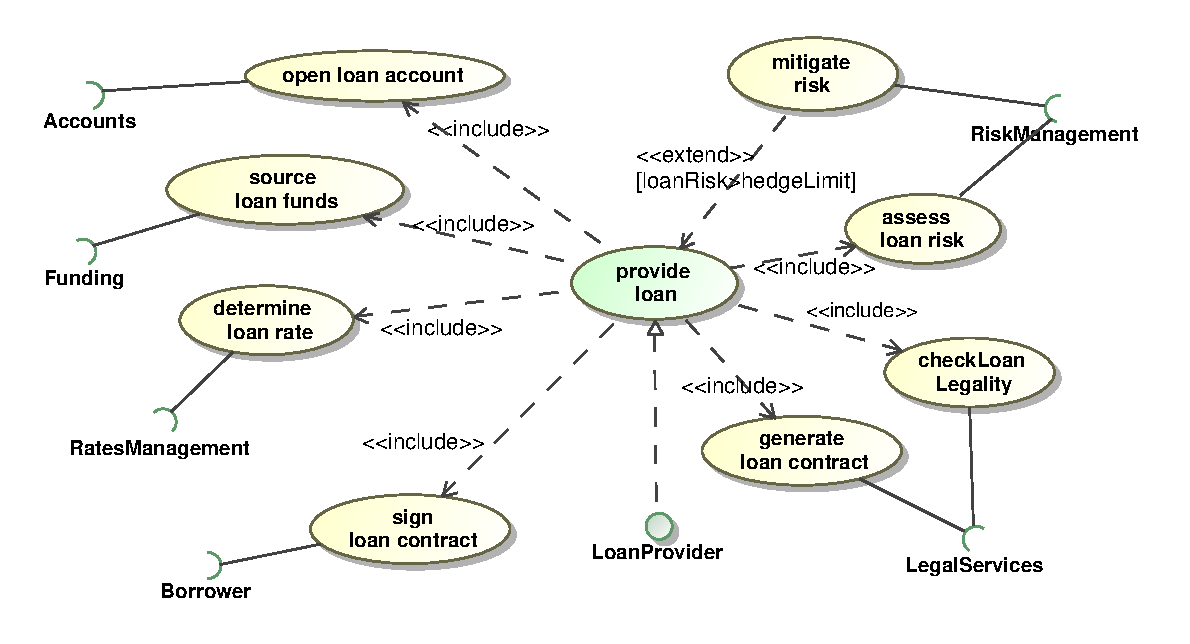
\epsfig{file=provideLoanResponsibilityAllocation.eps, scale=0.6}
  \caption{Responsibility identification and allocation.}
  \label{fig:provideLoanResponsibilityAllocation}
\end{figure}

Next one specifies how the business process is assembled across these services
providers. Optionally one could first look at a typical scenario using a
sequence diagram as is shown in figure
\ref{fig:provideLoanSuccessScenario}.


\begin{figure}
  \centering
  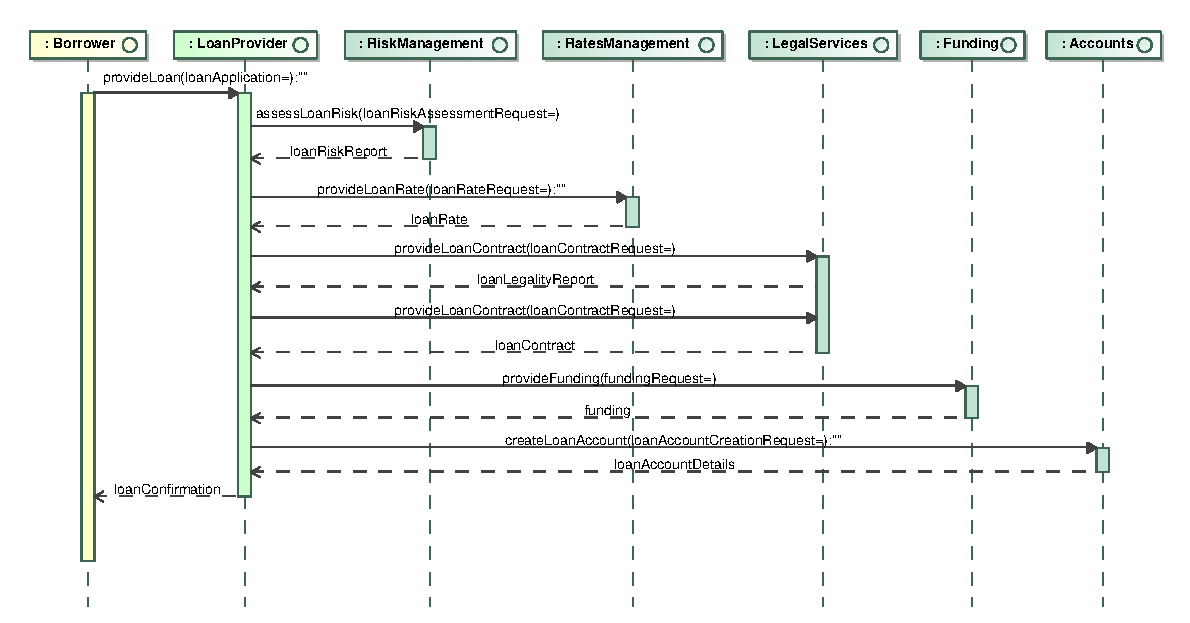
\epsfig{file=provideLoanSuccessScenario.eps, scale=0.6}
  \caption{Business process scenario scenario.}
  \label{fig:provideLoanSuccessScenario}
\end{figure}

Often business analysts may choose to omit the sequence diagram and specify the
full business process directly via an activity diagram. The UML tool feeds the
services required with their inputs and outputs into the respective
services contracts as shown in figure \ref{fig:provideLoanBusinessProcess}.
URDAD assumes that the higher level object, the training
provider, is the work flow controller which generates and issues the services
requests to the individual service providers for this level of granularity. The
subject from which the service is requested is, by default, chosen for the work
flow controller.

\begin{figure}
  \centering
  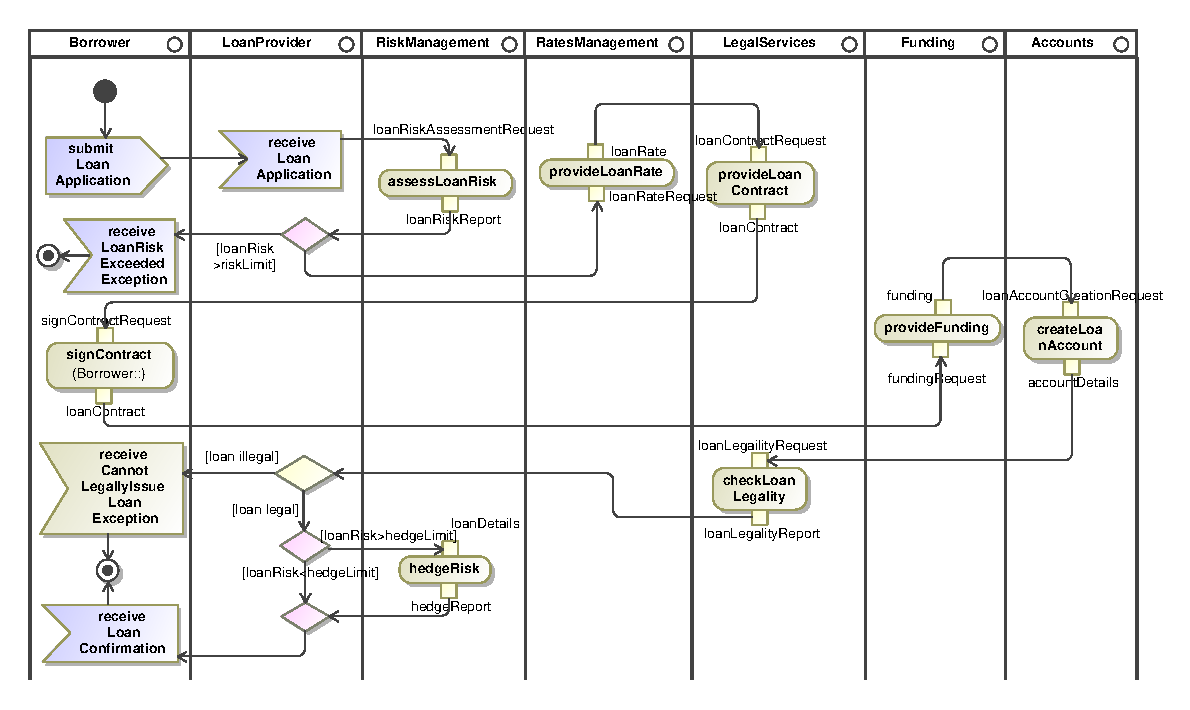
\epsfig{file=provideLoanBusinessProcess.eps, scale=0.6}
  \caption{Full business process for current level of granularity.}
  \label{fig:provideLoanBusinessProcess}
\end{figure}

In figure \ref{fig:provideLoanCollaborationContext} we project out the collaboration context
which represents the static structure within
which the collaboration is executed. It shows the services required from each service
provider together with the message paths required between them.

\begin{figure}
  \centering
  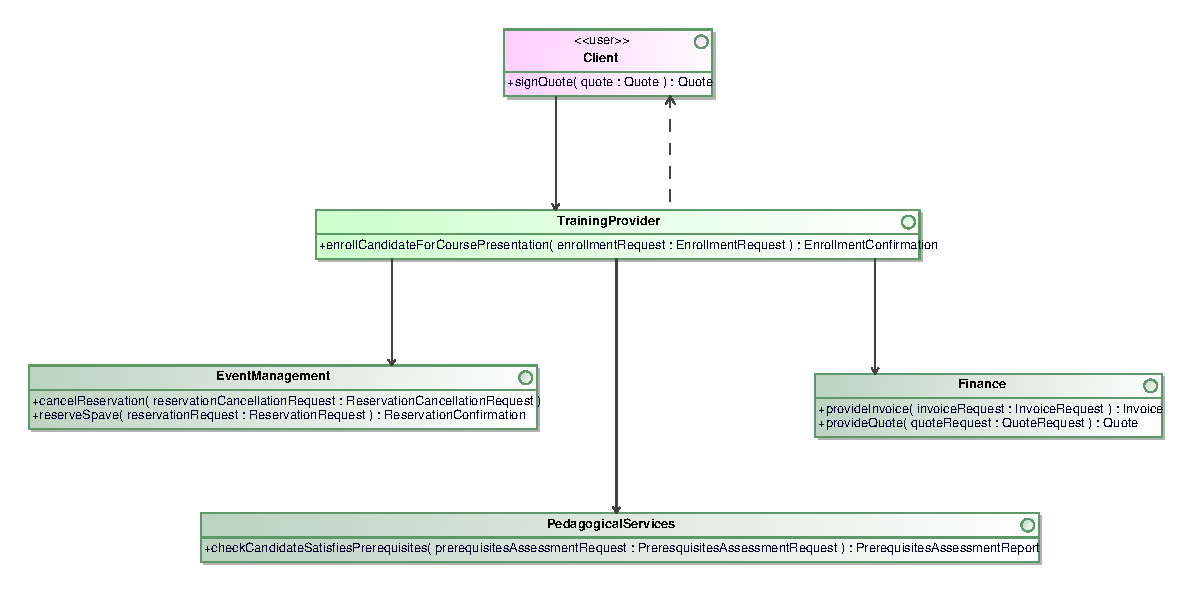
\epsfig{file=collaborationContextEnrollCandidate.eps, scale=0.6}
  \caption{Collaboration context for provide loan use case.}
  \label{fig:provideLoanCollaborationContext}
\end{figure}


%=========================================================

\subsection{Tying up use cases and services}

UML does not have a dedicated notation for just a service, though commonly
use cases are used for this purpose. In URDAD one ties up a particular use case
with a particular service by inserting a realization relationship between them.

%=========================================================

\subsection{Transition to next lower level of granularity}

In order to go over to the next lower level of granularity, one selects one
service provider (e.g.\ RiskManagement) from the current level of granularity as new
subject and one of its services (e.g.\ assessLoanRisk) for the subject the use case.

We start every level of granularity by an analysis stage where we first elicit the next level functional requirements as shown in figure figure \ref{fig:assessLoanRiskFunctionalRequirements}.

\begin{figure}
  \centering
  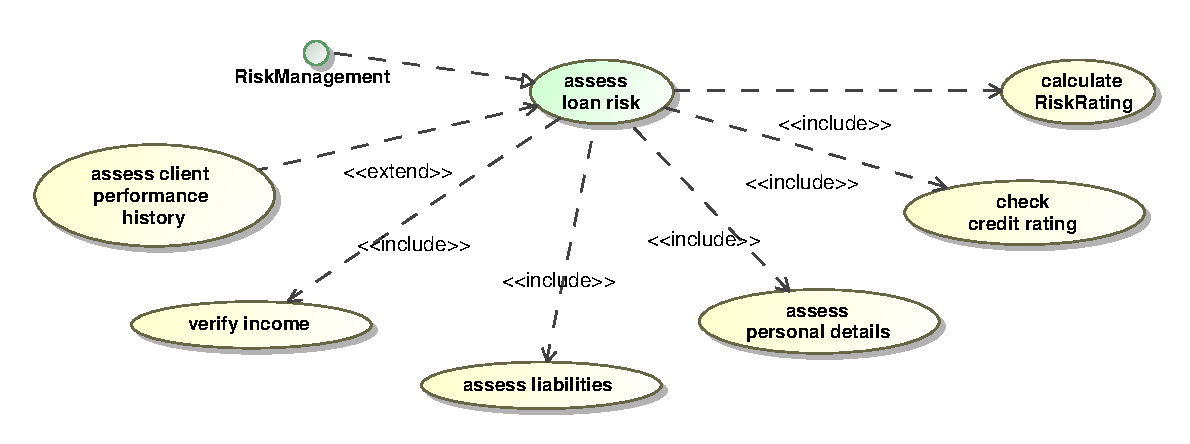
\epsfig{file=assessLoanRiskFunctionalRequirements.eps, scale=0.6}
  \caption{Lower level functional requirements.}
  \label{fig:assessLoanRiskFunctionalRequirements}
\end{figure}

The business process of the previous level of granularity will provide
the user work flow and we can directly go on to specify any new value objects
and the services contract.

This lower level use case is then taken through the business process design for this
lower level of granularity which will yield the PIM contributions for this level of granularity.
The process is repeated until the processes for all responsibility domains falling within
the scope of the subject (e.g.\ organization) have been fully specified.